\subsection{Construction du troisième parcours différencié en sixième}
\subsubsection*{Evaluation diagnostique}\label{Eval_diag_ju}
\begin{figure}[!h]
	\center{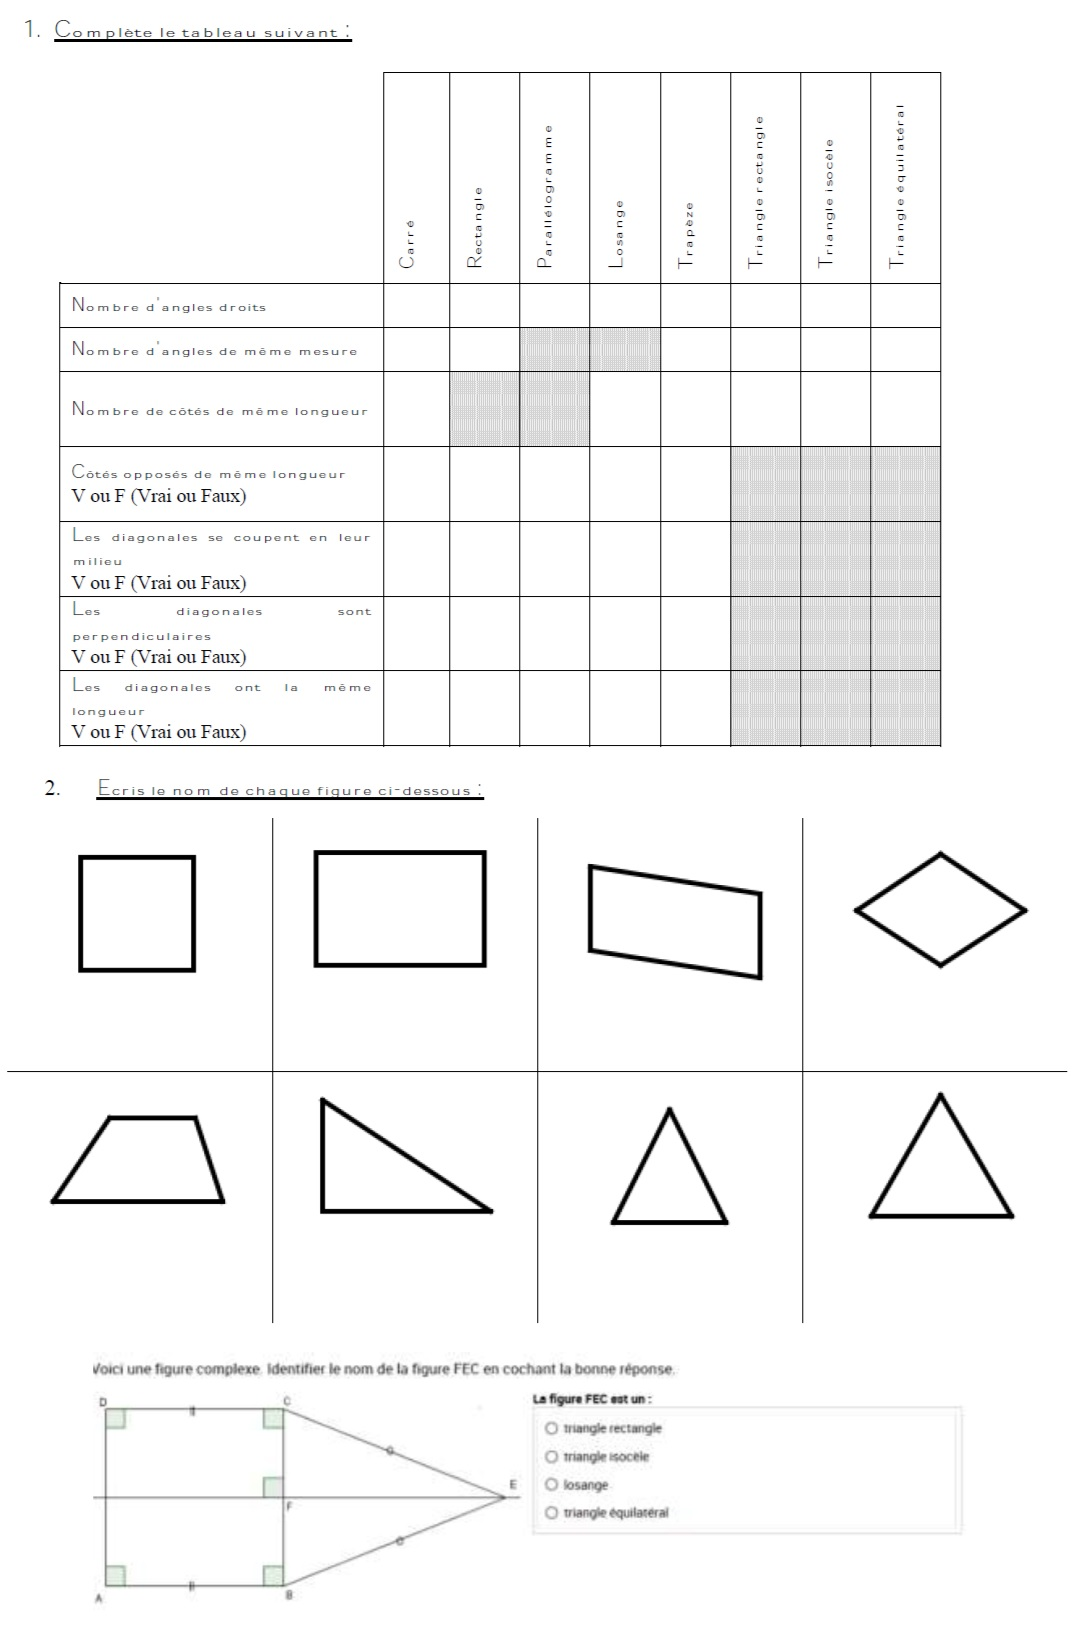
\includegraphics{img/eval_diag_julia.jpg}}
	\caption{Evaluation diagnostique}
\end{figure}
\subsubsection*{Productions d'élèves}
\begin{figure}[!h]
	\centering
	\subfloat[copie n°1]{{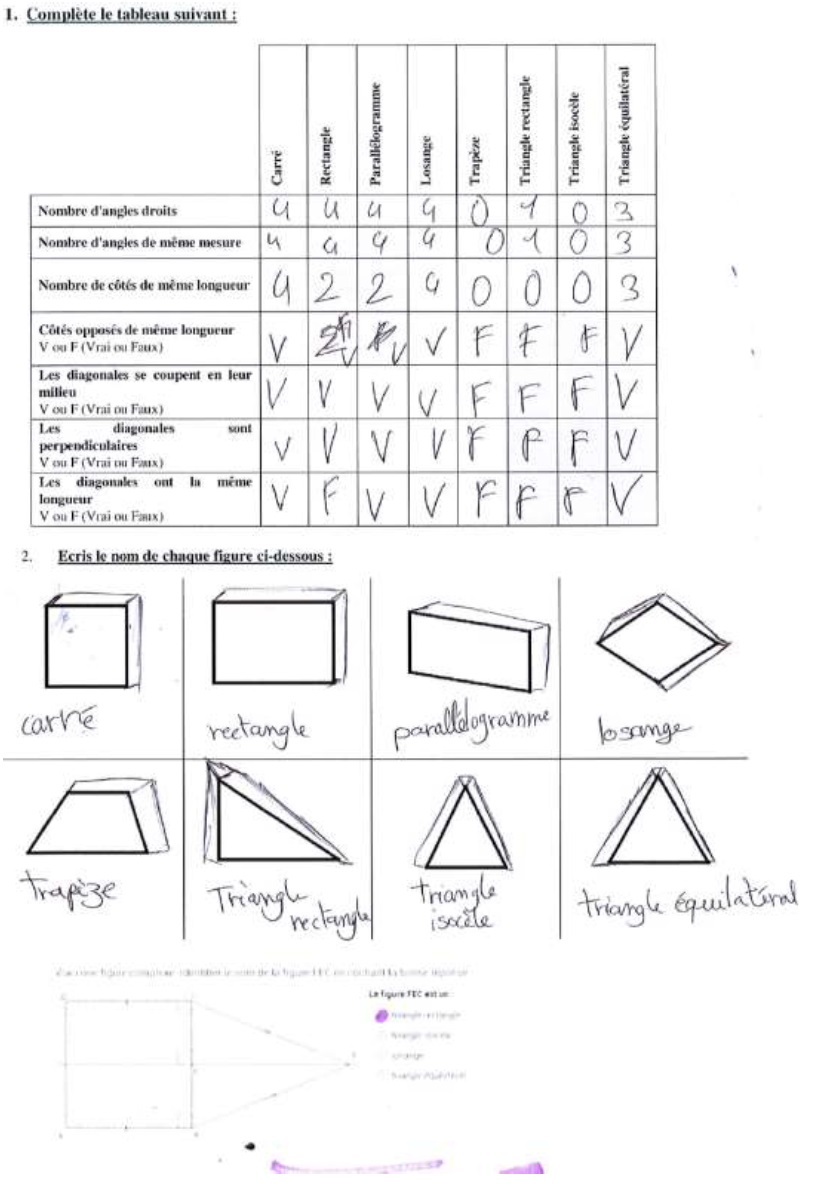
\includegraphics[scale=0.4]{img/copie1_eval_diag_ju.jpg}}}
	\qquad
	\subfloat[copie n°2]{{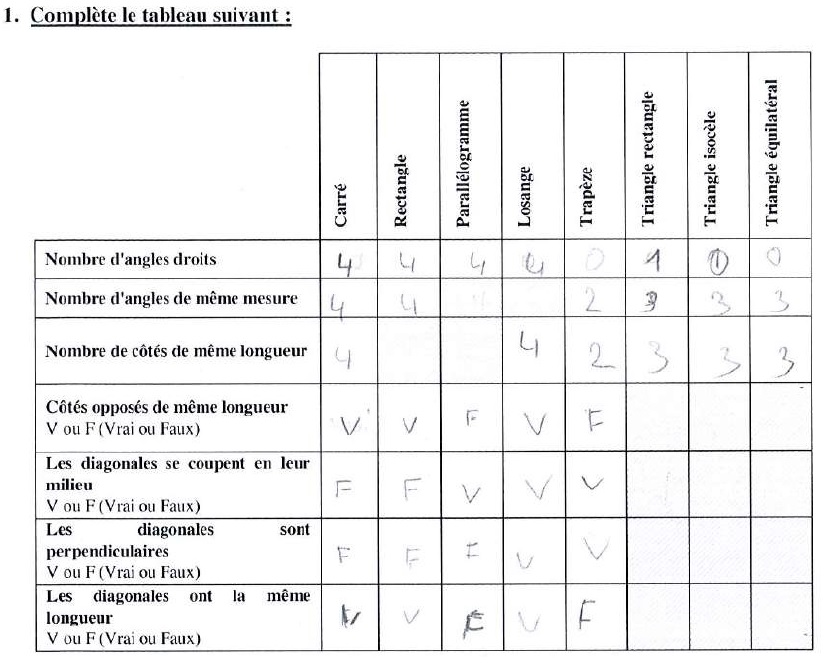
\includegraphics[scale=0.5]{img/copie2_eval_diag_ju.jpg}}}
	\qquad
	\subfloat[copie n°3]{{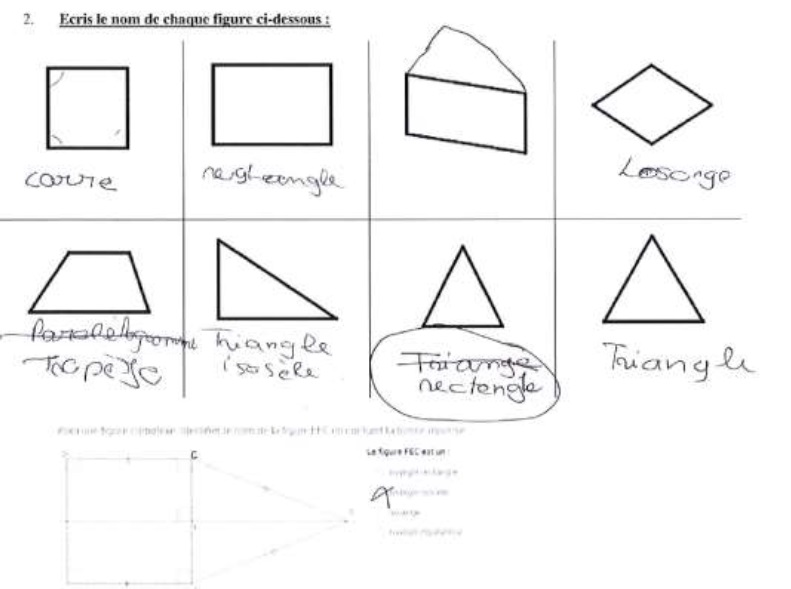
\includegraphics[scale=0.5]{img/copie3_eval_diag_ju.jpg}}}
	\caption{Evaluations d'élèves}
	\label{fig:Eval_diag_copies}
\end{figure}
\subsubsection*{Analyse des productions d'élèves}
\begin{figure}[!h]
	\centering
	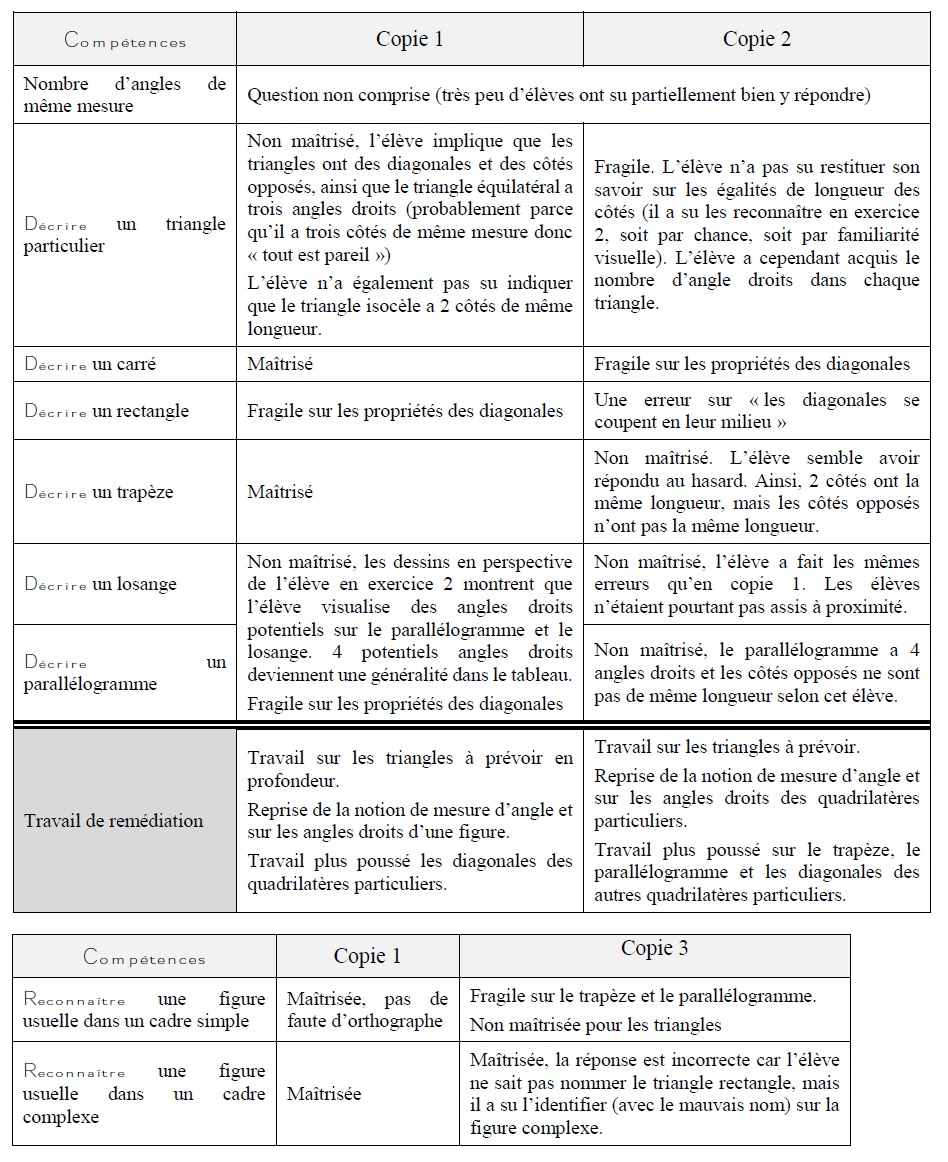
\includegraphics[scale=0.75]{img/Analyse_eval_diag_ju.jpg}
	\caption{Analyse des évaluations}
\end{figure}
\subsubsection*{Parcours différenciés}\label{parcours_diff3}
\textbf{\color{red} Note : Ajouter les parcours différenciés ICI avec le lien de chacun avec l'analyse diagnostique\\
Note 2 : Les annexes ne sont pas au bon endroit}
\subsubsection*{Supports des parcours différenciés}
Lien support vidéo\\
Support "fiche aide"\\
Grille projetée au tableau pour les tuteurs et tutorés.